\documentclass[11pt,a4paper]{article}
\newcommand{\guideshort}{Detailed user guide}
% Shared typesetting for the two source-grounded VPE teaching guides.
\usepackage[a4paper,margin=23mm,headheight=15pt]{geometry}
\usepackage{fontspec}
\setmainfont{Liberation Serif}
\setsansfont{Liberation Sans}
\setmonofont{Liberation Mono}
\usepackage{xcolor,graphicx,booktabs,tabularx,longtable,array}
\usepackage{listings,hyperref,tikz}
\usetikzlibrary{arrows.meta,positioning}
\definecolor{vveblue}{HTML}{174A70}
\definecolor{vvelight}{HTML}{F1F5F8}
\definecolor{vvegreen}{HTML}{266547}
\hypersetup{colorlinks=true,linkcolor=vveblue,urlcolor=vveblue,
  pdfauthor={Vienna Physics Engine},pdfsubject={Source-grounded beginner teaching edition}}
\setlength{\parindent}{0pt}
\setlength{\parskip}{6pt plus 1pt}
\setlength{\emergencystretch}{3em}
\sloppy
\renewcommand{\arraystretch}{1.18}
\makeatletter
\def\ps@vve{%
  \def\@oddhead{\small\sffamily Vienna Physics Engine\hfil\guideshort}%
  \let\@evenhead\@oddhead
  \def\@oddfoot{\small\sffamily Teaching edition / 16 October 2026\hfil\thepage}%
  \let\@evenfoot\@oddfoot}
\makeatother
\pagestyle{vve}
\lstdefinestyle{vvecpp}{language=C++,basicstyle=\ttfamily\small,
  keywordstyle=\color{vveblue}\bfseries,commentstyle=\color{vvegreen},
  stringstyle=\color{vvegreen},backgroundcolor=\color{vvelight},
  breaklines=true,breakatwhitespace=false,columns=fullflexible,
  keepspaces=true,showstringspaces=false,tabsize=4,
  frame=single,rulecolor=\color{vvelight},framesep=6pt,
  xleftmargin=6pt,xrightmargin=6pt,aboveskip=8pt,belowskip=8pt,
  morekeywords={import,requires,concept,constexpr,consteval,nodiscard}}
\lstset{style=vvecpp}
\newcommand{\api}[1]{{\ttfamily\small\detokenize{#1}}}
\newcommand{\source}[1]{\par\smallskip{\raggedright\footnotesize\sffamily\color{vveblue}Source: \nolinkurl{#1}.\par}}
\newcommand{\lesson}[1]{\clearpage\section{#1}}
\newenvironment{remember}{\begin{quote}\small\textbf{Remember. }}{\end{quote}}
\newenvironment{tryit}{\begin{quote}\small\textbf{Try it. }}{\end{quote}}
\newcommand{\guidecover}[3]{%
 \begin{titlepage}\sffamily\color{vveblue}
 {\large Vienna Physics Engine\par}\vspace{20mm}
 {\Huge\bfseries #1\par}\vspace{8mm}
 {\Large #2\par}\vspace{12mm}
 \color{black}{\large #3\par}\vfill
 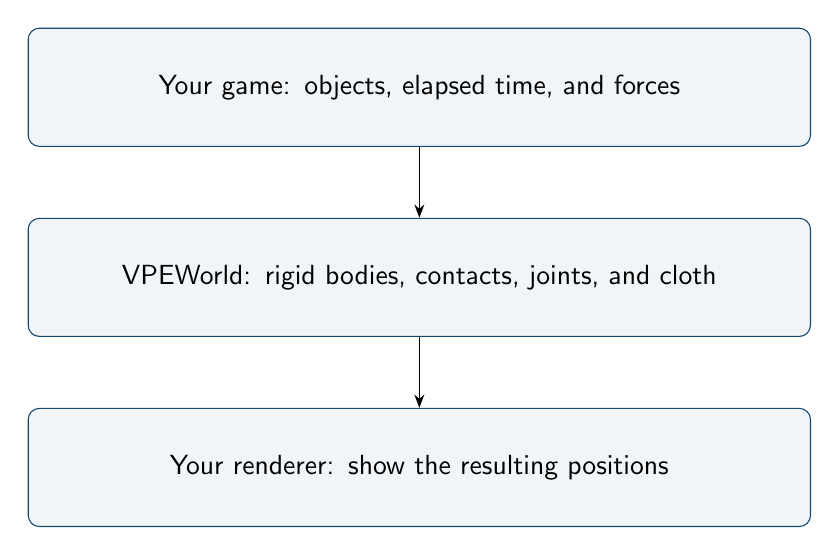
\begin{tikzpicture}[node distance=9mm,every node/.style={draw=vveblue,rounded corners,fill=vvelight,text width=0.8\linewidth,align=center,minimum height=15mm,font=\sffamily}]
 \node (game) {Your game: objects, elapsed time, and forces};
 \node (engine) [below=of game] {VPEWorld: rigid bodies, contacts, joints, and cloth};
 \node (result) [below=of engine] {Your renderer: show the resulting positions};
 \draw[-{Stealth}] (game)--(engine);
 \draw[-{Stealth}] (engine)--(result);
 \end{tikzpicture}\vfill
 {\normalsize Updated 16 October 2026\par}
 {\small Source baseline: debf892.\par}
 {\small Complete examples are checked against this source; excerpts state their context.\par}
 \end{titlepage}}

\hypersetup{pdftitle={Vienna Physics Engine - Detailed user guide}}
\begin{document}
\guidecover{Detailed user guide}{Physics explained step by step}{Learn the basic ideas, follow a simulation through its steps, and connect rigid bodies, joints and cloth to a game. Includes complete console exercises and current implementation details.}
\tableofcontents
\lesson{How to use this manual}
This manual starts with the vocabulary and reasoning a first-time physics user needs. The middle explains how VPE works. The later sections turn those details into small game features. Read the beginner quickstart for the fastest first run; return here when you want to understand each choice.

You should know how to declare a variable, call a function and write a loop in C++. You do not need a physics course, a Vulkan background or experience writing a solver. New terms are explained before they matter. A code listing with a full \api{main} function is a complete console program. Other listings are fragments and say which existing values they use.

This teaching edition follows source commit \api{debf892}, checked on 16 October 2026. The implementation lives mainly in \api{modules/VPE.ixx}. Older comments and build paths sometimes mention VVE V3; that is historical naming. The current graphics module is \api{VVEngine}, and the physics module remains \api{VEPhysicsEngine}.

The useful learning order is: one falling cube, a safe owner, a movement callback, one collision event, one joint, then a small cloth. Keep each small program so you can tell which addition caused a problem. You can use VPE with another renderer or no renderer at all.
\lesson{Five ideas before the first formula}
A simulation stores a simplified description of a world. It advances that description in small time intervals. It cannot inspect the picture on screen to discover what should collide. You explicitly give it collision shapes, starting positions and physical properties.

A rigid body is an object whose shape does not bend. A falling crate can move and rotate while the crate itself stays the same shape. Cloth is different: each part can move relative to the other parts. A joint is a rule connecting rigid bodies, such as the hinge of a door.

A position tells where an object is. Velocity tells how fast position changes. Acceleration tells how fast velocity changes. If a body moves at two metres per second for half a second, it travels about one metre. Gravity is acceleration downward; it gradually changes velocity rather than instantly setting a position.

A collision shape is a simple mathematical boundary. A detailed statue may use a few simple convex shapes even when its visible model contains thousands of triangles. The visible model helps the player see the statue; the collision shapes let the engine calculate contacts. Neither is created automatically from the other.

The physics world owns its lists of bodies and constraints. Your game owns meaning: which object is a player, whether a collision causes damage, and when a door unlocks. Callbacks carry results from the numerical world into your game rules and visible objects.
\lesson{Read the C++ without guessing}
\api{using W = vpe::VPEWorld;} is a short local name. \api{W::Body} means the \api{Body} class inside that world class. The \api{::} operator selects a name in a namespace or class. The \api{->} operator accesses an object through a pointer.

\api{std::make_shared<W::Body>(...)} constructs a body and returns a pointer that shares ownership. Copying that pointer keeps the same body alive; it does not create another body. The world stores a copy when you add the body. Removing it from the world does not destroy it if your game still holds a shared pointer.

\api{&owner} takes the address of a game object. It gives VPE an identity to look up, not permission to delete the object. \api{nullptr} means no pointed-to object; VPE reserves that owner for the built-in ground. A lambda, written \api{[captures](parameters) { ... }}, is a small function. Its captures provide data when it is called later.

\api{std::move(gravity)} permits moving a value into storage. Do not read a moved-from value expecting its previous contents; create or assign a new value first. The \api{1.0_real} suffix creates a number in the engine's configured number type. Ordinary values like 1 and 0 in a vector constructor can convert to that type.

The line \api{import VEPhysicsEngine;} imports a compiled C++ module. Standard headers in these examples come before it. CMake must know the module dependency, compiler and build options. Copying a compiled module file from an unrelated compiler or build configuration is not a reliable way to import it.
\lesson{Build the smallest useful project}
Start without rendering. That removes window, GPU and shader setup from your first physics exercise. The physics library itself uses C++23 and its bundled GLM headers. A suitable C++ module compiler, CMake 3.28 or newer and Ninja are the basic tools. Linux uses Clang and libc++; on Windows use the repository's supported Visual Studio toolchain and script.

Make a new game folder beside the VPE repository. The relative path in this complete \api{CMakeLists.txt} assumes those two folders are neighbours:\begin{lstlisting}
cmake_minimum_required(VERSION 3.28)
project(FirstPhysics LANGUAGES CXX)
set(CMAKE_CXX_EXTENSIONS OFF)
set(VPE_BUILD_EXAMPLES OFF CACHE BOOL "" FORCE)
set(VPE_BUILD_TESTS ON CACHE BOOL "" FORCE)
# This game folder is beside ViennaPhysicsEngine.
add_subdirectory(../ViennaPhysicsEngine vpe-build)
add_executable(first_physics main.cpp)
target_link_libraries(first_physics PRIVATE
    ViennaPhysicsEngine::ViennaPhysicsEngine)
\end{lstlisting}
Put the complete falling-body program from the later section in \api{main.cpp}. These commands explicitly select Clang 18 for Linux:\begin{lstlisting}
cmake -S . -B build -G Ninja -DCMAKE_BUILD_TYPE=Release \
    -DCMAKE_CXX_COMPILER=clang++-18
cmake --build build
ctest --test-dir build/vpe-build --output-on-failure
\end{lstlisting}
On Windows, configure from a Developer PowerShell and omit the Clang compiler option. On macOS, select the module compiler from the platform README. Choose it at the first configuration of a fresh directory; an existing module build must not mix compilers.

The first command creates build rules. The second compiles and links. CTest runs the registered physics checks in the VPE build subtree. Your own executable is an additional target and must also be run. On a multi-configuration setup add \api{--config Release} when building and \api{-C Release} when running CTest.

For the repository scripts, \api{--without-vve} selects standalone mode. For the graphical example, follow the platform README and keep VVE, compiler, standard library, configuration and module options compatible. Start by running the existing graphical example before changing its integration code.
\source{CMakeLists.txt; tests/CMakeLists.txt; README.md; build_linux.sh; build_macos.sh; build_windows.cmd}
\lesson{A glossary with small examples}
\textbf{Body}: the physical state of one rigid object, including position, rotation, speed and mass. A crate's visible mesh is a separate object.

\textbf{World space}: the coordinate system for the whole scene. \textbf{Local space}: coordinates relative to one object. A local point on the end of a rotating beam moves through world space as the beam turns. Member suffixes W and L distinguish the two.

\textbf{Inverse mass}: 1 divided by mass. A two-kilogram body has inverse mass 0.5. The special value zero means immovable; do not calculate 1 divided by zero to construct it.

\textbf{Contact}: the solver's description of two touching shapes. \textbf{Impulse}: a change in momentum used to respond to a contact or a joint. \textbf{Constraint}: a rule that the solver tries to satisfy, such as keeping a hinge anchor together.

\textbf{Fixed step}: a small interval used for the numerical calculation. \textbf{Frame}: one update of the application or renderer. One frame may contain no fixed physics steps, one step or several steps. \textbf{Residual time}: the fraction left after whole fixed slots have been consumed.

\textbf{Compliance}: how easily a cloth constraint gives way. More compliance means softer cloth. \textbf{Damping}: reduction of movement over time. \textbf{Restitution}: a material's bounce response. \textbf{Friction}: resistance to sliding at a contact.
\clearpage\part{The parts you use}
\lesson{What the engine does for your game}\label{vpe-core-1}
It calculates movement. Drawing is someone else's job. VPE calculates how solid objects and cloth move and bump into each other. Your game tells it which objects exist, where they start and which forces push them. Then the engine moves time forward. After each update it calls your callbacks, so your game can move the visible objects on screen.

\begin{center}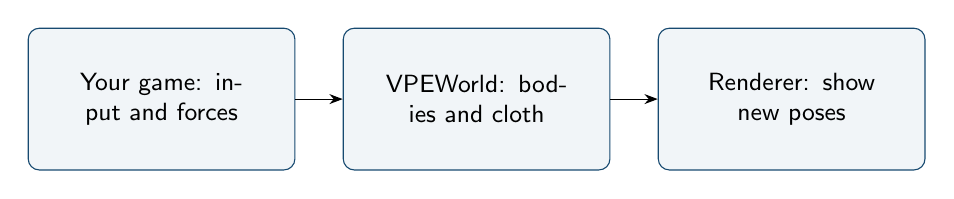
\begin{tikzpicture}[node distance=6mm,every node/.style={draw=vveblue,rounded corners,fill=vvelight,text width=0.26\linewidth,align=center,minimum height=18mm,font=\small\sffamily}]
\node (a) {Your game: input and forces};\node (b) [right=of a] {VPEWorld: bodies and cloth};\node (c) [right=of b] {Renderer: show new poses};
\draw[-{Stealth}] (a)--(b);\draw[-{Stealth}] (b)--(c);
\end{tikzpicture}\end{center}

You start with import VEPhysicsEngine;. All classes are in the namespace vpe. You simply create a vpe::VPEWorld object. There is no setup function, no window and no main loop inside the engine: your game decides when to call it.

\textbf{Job}: Who does it

\textbf{Mass, speed, forces, collisions and joints}: ViennaPhysicsEngine

\textbf{Cloth movement and the new cloth corner positions}: ViennaPhysicsEngine

\textbf{Loading 3D models, textures and materials}: Your game, or the Vienna Vulkan Engine (VVE)

\textbf{Input, game rules and when to update}: Your game

\textbf{Drawing on the screen (graphics card)}: VVE or another renderer

\subsection*{A useful picture to keep in mind}
The world stores the physics state. A Body is the physical side of an object. Your game object is the owner of that body and also has a visible side. These are three different things that belong together.
\source{modules/VPE.ixx; modules/VPE.cpp; examples/physicsexample/physicsexample.cpp}

\lesson{The classes at a glance}\label{vpe-core-2}
Which classes you call, and which ones only help the engine. All classes live inside VPEWorld, so their full names look like vpe::VPEWorld::Body.

\textbf{Class}: What it is for

\textbf{VPEWorld}: You use it. Holds everything; add and remove objects; tick moves time forward.

\textbf{Body, Force}: You use them. A solid object, and a push that acts on it.

\textbf{Polytope}: You use it. A convex collision shape. The ready-made cube is g\_cube.

\textbf{BallSocketJoint, HingeJoint,}: You use them. Connections between two bodies (section~\ref{vpe-core-7}). SliderJoint, FixedJoint, DistanceConstraint

\textbf{Cloth}: You use it. A soft object made of triangles (section~\ref{vpe-core-8}).

\textbf{Vertex, Edge, Face}: Helpers: the corners, edges and faces that make up a Polytope.

\textbf{Contact, ContactPoint}: Helpers: the engine's notes about a collision. You do not create them.

\textbf{SatQuery, EdgeQuery, FaceQuery}: Helpers for the exact collision test (section~\ref{vpe-core-14}).

\textbf{ClothMassPoint, ClothTriangle,}: Helpers: the inner parts of a cloth. Cloth makes them for you. ClothConstraint

\textbf{MapWrapper}: Helper: the list in which the world stores its bodies (section~\ref{vpe-core-4}).

Many member variables are public, so you can change them directly. That does not mean every change is safe. Use the functions (addBody, setForce and so on) when they exist. Section~\ref{vpe-core-24} explains what to do when you change values by hand.
\source{modules/VPE.ixx; modules/VPE.cpp; examples/physicsexample/physicsexample.cpp}

\lesson{Numbers, units and directions}\label{vpe-core-3}
What positions, rotations and masses mean. The engine has its own short names for number types. You can use them without vpe:::

\textbf{Name}: Meaning

\textbf{real}: A decimal number (normally float).

\textbf{glmvec3}: A 3D vector: x, y, z. Used for positions, speeds and forces.

\textbf{glmquat}: A rotation (quaternion). No rotation is glmquat\{1,0,0,0\}.

\textbf{glmmat4}: A 4x4 matrix, used to place an object in the world.

2.5\_real                      Writes a number in the engine's real type.

Member names end with a letter that tells you the space: W means world space (the whole scene), L means local space (relative to the body itself). For example m\_positionW is the position in the world, and m\_orientationLW turns local directions into world directions.

\textbf{Value}: Meaning

m\_positionW, m\_linear\_velocityW                       Where the body is, and how fast it moves.

m\_angular\_velocityW                                   How fast it spins, in radians per second.

m\_scale                                               The size of the body.

m\_mass\_inv                                            Inverse mass. 0 means the body never moves.

Up is +y. The floor is the flat plane at y = 0. Two CMake options change the number setup: VPE\_DOUBLE\_ACCURACY uses double instead of float, and VPE\_FORCE\_LEFT\_HANDED changes the coordinate system. Both are off by default. Build the engine and your game with the same options.

\subsection*{A simple rule for units}
Use 1 unit = 1 meter, time in seconds and mass in kilograms everywhere. If your 3D models use other units, convert them once when you load them. Test with one falling cube before you build a big scene.
\source{modules/VPE.ixx; modules/VPE.cpp; examples/physicsexample/physicsexample.cpp}

\lesson{The world and how it stores objects}\label{vpe-core-4}
Adding, finding and removing bodies. The world finds a body by its owner pointer. The owner is usually a pointer to your game object. The engine does not know what type it is (it is a void*); it only uses the address as a name tag. So every body needs its own owner address, and that address must not change. The built-in floor uses nullptr as its owner.

\textbf{Function}: What it really does

\textbf{addBody(body)}: Puts the body into the world. It does not check whether the owner is already used.

\textbf{getBody(owner)}: Finds a body. It returns a pair; the body is in .second.

\textbf{eraseBody(body)}: Removes the body, calls its erase callback, and also removes all joints that use it.

\textbf{eraseBody(owner)}: Removes the body too, but does not remove its joints. Prefer the version above.

\textbf{clear()}: Removes all bodies and joints. Cloth is not removed: use clearCloths() for that.

Bodies are stored in a MapWrapper. It looks like a map, but inside it is a simple list, so finding a body walks through the list. If you look up an owner that is not there, it throws an exception instead of adding an empty entry like std::unordered\_map would. If two bodies share one owner, finding and removing them becomes unreliable. The world and the joints hold bodies with shared\_ptr. But a body only keeps plain pointers to its world and its shape. So a body does not keep the world, its shape or your game object alive: you must do that.

\subsection*{How to remove a body safely}
Store the body's shared\_ptr in your game object and remove it with eraseBody(body). If you decide to remove it inside a callback, only note it in a list, and remove it after tick has returned.
\source{modules/VPE.ixx; modules/VPE.cpp; examples/physicsexample/physicsexample.cpp}

\lesson{Bodies and forces}\label{vpe-core-5}
The two classes you use most. A Body has a position, rotation, speed, spin, inverse mass, bounciness, friction and a list of forces. It also stores some values the engine calculates for itself, such as matrices and inertia.

\begin{lstlisting}
using W = vpe::VPEWorld;
auto body = std::make_shared<W::Body>(
    &world, "crate", &owner, &W::g_cube,                       // world, name, owner, shape
    glmvec3{1,1,1}, glmvec3{0,4,0},                              // size, position
    glmquat{1,0,0,0},                                            // rotation
    glmvec3{0,0,0}, glmvec3{0,0,0},                              // speed, spin
    1.0_real, 0.2_real, 0.8_real);                               // inverse mass, bounciness, friction
\end{lstlisting}

This fragment assumes an existing world and a stable owner. Everything after the position is optional. If you leave it out, the body has no rotation, no speed, inverse mass 0 (it does not move!), bounciness 0.2 and friction 1. The constructor makes the shape 0.1 percent bigger as a safety margin and calculates the inertia for you.

\textbf{Member}: How to use it

\textbf{setForce(id, force)}: Adds a force with a number (ID). Using the same ID again replaces the old force.

\textbf{removeForce(id)}: Removes that force.

m\_on\_move                                            Your callback: called after the body moved. You get a time value and the body.

m\_on\_erase                                           Your callback: called when the body is removed, so you can remove the visible object.

\api{updateMatrices()} and \api{inertiaTensorL()}: recalculate dependent values after direct edits.

\api{Body::computeModel(pos, rot, scale)}: build the matrix that places an object.

A Force has four fields: m\_accelW is an acceleration (it is not divided by the mass, so all bodies fall equally fast); m\_forceW is a force in the world (divided by the mass); m\_forceL and m\_positionL are a force on a point of the body, which also makes it spin.

\subsection*{Gravity is not automatic}
The world has the value c\_gravity (-9.81), but a new body does not use it by itself. Add it: body->setForce(0ul, W::Force\{\{0, world.c\_gravity, 0\}\});
\source{modules/VPE.ixx; modules/VPE.cpp; examples/physicsexample/physicsexample.cpp}

\lesson{Shapes and collisions}\label{vpe-core-6}
The shape you see and the shape that collides are different things. A Polytope is the collision shape of a body. It is made of corners (vertices), edges and flat faces, and it knows which ones are connected. The ready-made VPEWorld::g\_cube is a cube. Many bodies can share it: each body has its own m\_scale, so the same cube can be a small box or a long plank. The exact collision test works only for convex shapes (no dents or holes). A 3D model you load, for example a chair or a car, is usually not convex and cannot be used directly. Instead, you approximate it with one or more convex shapes, such as a few boxes.

\textbf{Helper}: What it stores

\textbf{Vertex}: One corner of the shape, and which edges and faces it belongs to.

\textbf{Edge}: Two corners and the two faces next to it.

\textbf{Face}: One flat side, its direction (normal) and its edges.

\textbf{Contact}: Two bodies that touch, and the touching points from this and the last step.

\textbf{ContactPoint}: One touching point and the pushes (impulses) used there.

The world creates contacts by itself. Your game normally learns about collisions through a collision callback (section~\ref{vpe-core-25}), not by reading contacts. Contacts are kept from one step to the next, so do not remove bodies or change shapes while the engine is running.

\subsection*{Keep shapes alive and unchanged}
The parts of a Polytope point to each other. If you copy it, or put it in a std::vector that grows later, those pointers break. Build a shape once, keep it in one place and keep it alive while bodies use it.
\source{modules/VPE.ixx; modules/VPE.cpp; examples/physicsexample/physicsexample.cpp}

\lesson{Joints}\label{vpe-core-7}
\textbf{Connect two bodies and choose how they may still move. Joint}: What stays connected; What can still move

\textbf{BallSocketJoint}: One shared point; Turning in all directions (like a shoulder)

\textbf{HingeJoint}: One shared point and an axis; Turning around that axis (like a door)

\textbf{SliderJoint}: Rotation and sideways position; Sliding along one axis (like a drawer)

\textbf{FixedJoint}: Position and rotation; Nothing: the bodies move as one

\textbf{DistanceConstraint}: The distance between the centers; Everything else (like a rod)

\begin{lstlisting}
using W = vpe::VPEWorld;
// support and door are bodies that were already added.
auto hinge = std::make_shared<W::HingeJoint>(
    support, door,
    glmvec3{0, 2, 0},     // the shared point, in world coordinates
    glmvec3{0, 1, 0});    // the hinge axis (must not be zero)
hinge->enableLimit(-0.5_real, 0.5_real);   // allowed angles, in radians
world.addConstraint(hinge);
\end{lstlisting}

Other constructors: BallSocketJoint(a, b, point), FixedJoint(a, b, point), SliderJoint(a, b, point, axis) and DistanceConstraint(a, b, distance).

A hinge limit is measured from the starting angle. The minimum must be smaller than the maximum, and 0 should be between them. Hinges and sliders can also have a motor: enableMotor(speed, maxForce) drives them at a speed, and disableMotor() stops it. Remove a joint with removeConstraint. A joint keeps its two bodies alive, because it holds them with shared\_ptr. Joined bodies still collide with each other: there is no switch to turn that off. Place their shapes so they do not block the movement you want.
\source{modules/VPE.ixx; modules/VPE.cpp; examples/physicsexample/physicsexample.cpp}

\lesson{Cloth}\label{vpe-core-8}
A soft object made from a triangle mesh. To make a cloth you give: the world, a name, an owner, a move callback, an erase callback, the corner positions, the triangles and the pinned positions. Three settings are optional. Unlike a Body, the callbacks are given to the constructor.

\textbf{Input or function}: Meaning

\textbf{vertices and triangle indices}: The mesh: corner positions, and three corner numbers per triangle.

\textbf{fixedPointsPositions}: Corners that are pinned and do not move. Use the same positions as in vertices.

\textbf{bendingCompliance (default 1)}: How easily the cloth bends. Bigger means softer. It is not a spring stiffness.

\textbf{substeps (default 4)}: How many small steps per physics step. Must be above 0.

\textbf{movementSimulation (default 0.8)}: How much of a movement you apply is simulated (section~\ref{vpe-core-18}).

\textbf{generateVertices()}: Returns the current corner positions, in the order you gave them.

\api{applyTransformation(matrix, simulate)}: move or turn the cloth.

\textbf{addCloth, getCloth, eraseCloth,}: Add, find and remove cloth. Cloth is stored apart from bodies. clearCloths

Corners within the implementation's position tolerance are joined into one physical point. A 3D model often has such doubled corners at its seams. generateVertices() still gives you one position per original corner, so your mesh keeps working. A cloth cannot be copied or moved in memory, because its parts point to each other: always create it with std::make\_shared. The constructor checks its input and throws an exception if something is wrong: a missing world, invalid numbers, a triangle index that does not exist, or a mesh with loose points. addCloth throws if the cloth is nullptr or if its owner is already used.

\subsection*{The engine does not draw the cloth}
It only gives you positions. Your renderer must copy them into the mesh, recalculate the normals if the material needs them, and upload everything to the graphics card.
\source{modules/VPE.ixx; modules/VPE.cpp; examples/physicsexample/physicsexample.cpp}

\clearpage\part{How the engine works inside}
\lesson{Files and starting values}\label{vpe-core-9}
What happens when you create a world. Almost the whole engine is in one file, modules/VPE.ixx. It contains the classes and also their code. The small file modules/VPE.cpp only has two math helper functions.

\begin{center}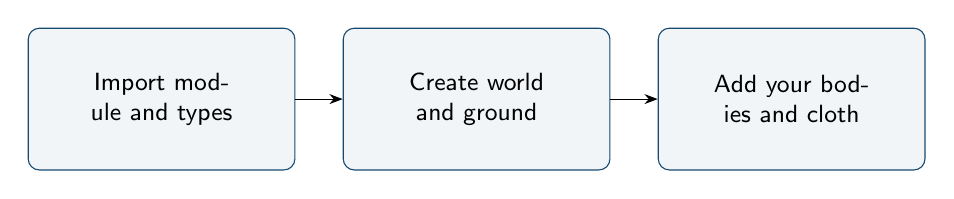
\begin{tikzpicture}[node distance=6mm,every node/.style={draw=vveblue,rounded corners,fill=vvelight,text width=0.26\linewidth,align=center,minimum height=18mm,font=\small\sffamily}]
\node (a) {Import module and types};\node (b) [right=of a] {Create world and ground};\node (c) [right=of b] {Add your bodies and cloth};
\draw[-{Stealth}] (a)--(b);\draw[-{Stealth}] (b)--(c);
\end{tikzpicture}\end{center}

The VPEWorld constructor itself is empty. All starting values come from the member variables. One of them is the floor: a very large, unmovable body with owner nullptr.

\textbf{Starting value}: What it means for you

60 steps per second (m\_sim\_frequency)                        The engine always moves in steps of 1/60 second.

m\_loops = 30                                                 Up to 30 rounds to solve contacts and joints in each step.

m\_solver = 0                                                 Which contact solver is used (section~\ref{vpe-core-15}).

Grid cell width 3 (m\_width)                                  Size of the cells used to find nearby bodies (section~\ref{vpe-core-13}).

\textbf{Floor at y = 0}: Always there. A floor you draw does not change it.

\textbf{No main loop}: Nothing happens until your game calls tick.

Create the world in a place where it stays, add your callbacks and bodies, and then start calling tick. Do not copy or move the world later: every body remembers the world's address.
\source{modules/VPE.ixx; modules/VPE.cpp; examples/physicsexample/physicsexample.cpp}

\lesson{One tick, step by step}\label{vpe-core-10}
Set a breakpoint in tick and step over these lines. tick first works out how many physics steps are due (section~\ref{vpe-core-11}). For each step it does this:

\textbf{Order}: What happens in one physics step

\textbf{1}: Broad phase: quickly find pairs of bodies that are near each other.

\textbf{2}: Narrow phase: test those pairs exactly and create or update contacts.

\textbf{3}: Warm start: reuse the pushes from the last step for contacts that still exist.

\textbf{4}: Change each body's speed using its forces.

\textbf{5}: Prepare the joints, then repeat up to 30 times: correct the speeds at contacts and joints.

\textbf{6}: Remember the old position, move each body with its new speed, update its matrices.

\textbf{7}: Move every cloth, in several small steps, including its contacts with bodies.

\textbf{8}: Apply the pushes the cloth gave to bodies, and update their matrices.

After all due steps are done, the world updates which grid cell each body is in. Then it calls the move callbacks of all bodies and all cloth. So your callbacks run once per tick, not once per step.

\subsection*{Where your own code fits}
Before tick: your game sets forces. During tick: the engine calculates and then calls your callbacks, which publish the new positions. After tick: your renderer draws. The engine never talks to the graphics card.
\source{modules/VPE.ixx; modules/VPE.cpp; examples/physicsexample/physicsexample.cpp}

\lesson{Time steps, leftover time and pausing}\label{vpe-core-11}
Why the engine moves in fixed steps. A game's frames are not all equally long. Physics is more stable when every step has the same length. So the engine collects the time you give it and does one fixed step of 1/60 second each time enough time has passed. In simple form:

\begin{lstlisting}
// Simplified version of what tick does:
current_time = last_time + dt;
while (current_time > next_step_time) {
    do_one_step(1/60 second);
    last_step_time = next_step_time;
    next_step_time += 1/60 second;
}
call_callbacks(current_time - last_step_time);                       // the leftover time
last_time = current_time;
\end{lstlisting}

Note the >: if you call tick(1.0/60.0) exactly once at the start, the time is equal, not greater, so no step happens yet. The next call then does the step. If a frame was slow, one tick does several steps to catch up. There is no limit. After a long pause or a stop in the debugger, a huge dt can make the engine work for a long time. Decide in your game what should happen: make dt smaller, skip the paused time, or catch up on purpose.

The move callback gets the leftover time: the time since the last step. You can use it to guess where the body is between two steps, so the motion looks smoother. Keep that guess separate from the real physics position.

\textbf{Thing to know}: Why

\textbf{Debug mode}: In SIMULATION\_MODE\_DEBUG, tick ignores dt. The example moves the clock itself and then calls tick(0).

m\_run does nothing                       The variable exists, but tick does not check it. To pause, do not call tick.

\textbf{Changing the step rate}: Setting m\_sim\_frequency alone does not change m\_sim\_delta\_time. Change both.
\source{modules/VPE.ixx; modules/VPE.cpp; examples/physicsexample/physicsexample.cpp}

\lesson{How forces become movement}\label{vpe-core-12}
First the speed changes, then the position. In each step, Body::stepVelocity adds up all forces of a body. Accelerations are added directly. Forces are multiplied by the inverse mass (heavy bodies speed up less). A force on a point of the body also makes it spin; the inertia decides how much.

\begin{center}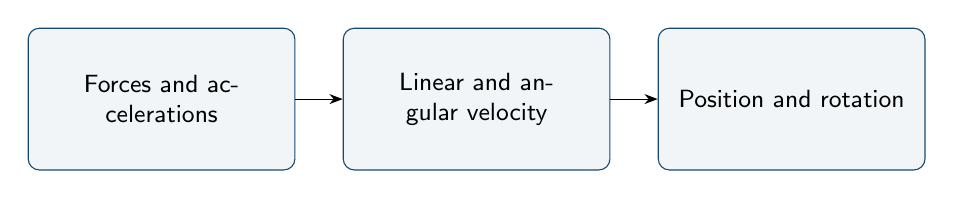
\begin{tikzpicture}[node distance=6mm,every node/.style={draw=vveblue,rounded corners,fill=vvelight,text width=0.26\linewidth,align=center,minimum height=18mm,font=\small\sffamily}]
\node (a) {Forces and accelerations};\node (b) [right=of a] {Linear and angular velocity};\node (c) [right=of b] {Position and rotation};
\draw[-{Stealth}] (a)--(b);\draw[-{Stealth}] (b)--(c);
\end{tikzpicture}\end{center}

A force stays until you remove or replace it. Gravity, added once, acts in every step. That is good for gravity, but bad for a jump: a jump force that stays would push the body up forever. For a one-time push, change the speed directly instead (section~\ref{vpe-core-24}).

\textbf{Stored value}: Why the engine needs it

\textbf{Inertia (local, and inverse in world space)}: How hard it is to make the body spin in its current rotation.

\textbf{Previous position and rotation}: Needed when cloth touches the body.

\textbf{Position and speed corrections}: Small fixes that push overlapping bodies apart. Not a game force.

\textbf{Resting counter and damping}: Lets bodies that lie still calm down instead of jittering.

\textbf{Model matrix and its inverse}: Turns the shape's corners into world positions for the collision test.

Body::stepPosition then moves the position and rotation using the speeds. Note: even when the example calls it on copies to guess a drawing position, it still updates some resting information of the body.

\subsection*{One place for the truth}
Do not move the visible object on its own while the physics body moves somewhere else. Change the physics body, and let the callback copy its position to the visible object.
\source{modules/VPE.ixx; modules/VPE.cpp; examples/physicsexample/physicsexample.cpp}

\lesson{Broad phase: finding nearby pairs}\label{vpe-core-13}
A quick filter before the exact test. Testing every body against every other body would be slow. So the engine puts the bodies on a flat grid, seen from above (x and z). Each body is in the cell where its center is. Only bodies in the same or a neighboring cell become a pair. Every body is also paired with the floor. Being a pair does not mean the bodies touch. The broad phase only says "these two might touch". The narrow phase (section~\ref{vpe-core-14}) checks it exactly.

\textbf{Situation}: What to watch out for

\textbf{Very large bodies}: Two big bodies can overlap while their centers are more than one cell apart. Then the pair is missed.

\textbf{Very fast bodies}: The engine checks at each step, not in between. A fast, thin object can pass through another.

\textbf{Negative coordinates}: Cells are computed by cutting off decimals, so cells next to 0 behave a bit differently.

\textbf{Several steps in one tick}: The cell of each body is updated only after all steps of the tick.

\textbf{Changing the cell width}: Bodies keep their old cells. You must sort them in again.

Choose a cell width (m\_width, default 3) that fits your object sizes. Bigger cells miss fewer pairs, but create more pairs to test.

\subsection*{Debugging a missed collision}
First check whether the two bodies ever became a pair. If not, the problem is the grid or the owners, and changing friction or other contact settings will not help.
\source{modules/VPE.ixx; modules/VPE.cpp; examples/physicsexample/physicsexample.cpp}

\lesson{Narrow phase: the exact test}\label{vpe-core-14}
From a possible pair to real touching points. For each pair, the engine first checks two spheres around the bodies. If the spheres do not touch, the bodies cannot touch either, and the pair is skipped. Otherwise the engine does an exact test called SAT (separating axis test). The idea of SAT: if you can find a direction in which the two shapes do not overlap, they do not collide. The engine tries the directions of all faces and of edge pairs. If none separates the shapes, they collide, and the engine calculates the touching points and how deep they overlap.

\begin{center}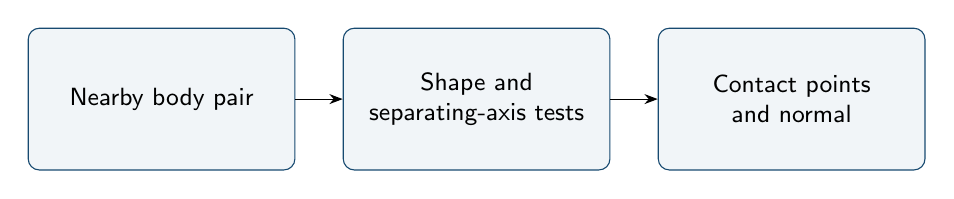
\begin{tikzpicture}[node distance=6mm,every node/.style={draw=vveblue,rounded corners,fill=vvelight,text width=0.26\linewidth,align=center,minimum height=18mm,font=\small\sffamily}]
\node (a) {Nearby body pair};\node (b) [right=of a] {Shape and separating-axis tests};\node (c) [right=of b] {Contact points and normal};
\draw[-{Stealth}] (a)--(b);\draw[-{Stealth}] (b)--(c);
\end{tikzpicture}\end{center}

The floor is a special case: the engine simply checks which corners of the body are below y = 0. Contacts are kept from step to step. The engine compares old and new touching points. This lets it reuse the pushes from the last step (warm starting), which makes stacks of boxes stable. Contacts that no longer touch are deleted. Your collision callback (section~\ref{vpe-core-25}) is called from here when a pair touches. It is not called in every step for bodies that lie still, and there are no separate "started touching" or "stopped touching" events.

\subsection*{Do not change the world inside a callback}
Collision callbacks run while the engine is going through its lists. Only write down what happened, and make your changes after tick has returned.
\source{modules/VPE.ixx; modules/VPE.cpp; examples/physicsexample/physicsexample.cpp}

\lesson{Solving contacts}\label{vpe-core-15}
Small pushes that stop bodies from sinking into each other. When two bodies touch, the engine gives each a short push, an impulse, at the touching point. An impulse changes the speed at once, and because it acts away from the center it can also change the spin. Both bodies get a push, in opposite directions. How much each one reacts depends on its mass and inertia.

\textbf{Setting or idea}: What it does

m\_solver = 0                                Default. Solves the push and the friction together.

m\_solver = 1                                Solves the push first and then the friction in two side directions.

\textbf{Push (normal impulse)}: Can only push, never pull, so touching bodies do not stick together.

\textbf{Friction}: Slows sliding. It can be at most the push times the friction value.

\textbf{Bounciness (restitution)}: How much a body bounces back.

m\_bias, m\_slop                              Push overlapping bodies apart; a tiny overlap (0.001) is allowed.

Warm starting (m\_use\_warmstart, on by default) starts with the pushes of the last step for contacts that still exist. This makes stacks stable with less work. The engine repeats the solving up to m\_loops (30) times per step. In normal (real-time) mode it also stops when one step's time (1/60 second) is used up, so a slow computer may do fewer rounds. In debug mode there is no time limit.

\subsection*{Same input does not always mean same result}
Because of the time limit, two computers can get slightly different results. Do not build networked multiplayer that needs exactly the same physics everywhere without testing this first.
\source{modules/VPE.ixx; modules/VPE.cpp; examples/physicsexample/physicsexample.cpp}

\lesson{Joints inside the solver}\label{vpe-core-16}
A joint is corrected again and again, together with contacts. Before the solving rounds, each joint prepares itself (setUp): it calculates where its connection points are now and how strongly it must correct. In each round, solveVelocity pushes the two bodies so the unwanted movement gets smaller. Contacts and joints are solved in the same rounds, so a mechanism and the ground it touches affect each other.

\textbf{Joint}: The error it tries to remove

\textbf{DistanceConstraint}: The centers are closer or farther apart than they should be.

\textbf{BallSocketJoint}: The two copies of the shared point have drifted apart.

\textbf{HingeJoint}: The shared point has drifted, or the bodies turn off the axis. Optional limits and motor.

\textbf{FixedJoint}: Any change in distance or rotation between the bodies.

\textbf{SliderJoint}: Sideways movement or rotation. Optional limits and motor along the axis.

When you create a joint, the shared point you give in world coordinates is stored in each body's own local coordinates. When the bodies move, the engine turns these local points back into world points and compares them. A limit only becomes active when the movement reaches it. Joints can shake or stretch when bodies have very different masses, when the connection point is in the wrong place, when contacts fight against the joint, or when there are too few solving rounds.

\subsection*{A good way to watch a joint in the debugger}
Set breakpoints in the joint constructor, in setUp and in solveVelocity. The local points stay the same; the world points, the error and the total push change.
\source{modules/VPE.ixx; modules/VPE.cpp; examples/physicsexample/physicsexample.cpp}

\lesson{How cloth is built and moved}\label{vpe-core-17}
From a mesh to a net of points. When you create a cloth, it first checks the mesh. Then it joins corners at the same position into one mass point and remembers which original corners belong to which point. Each triangle edge becomes a constraint that keeps two points at their distance. Extra bending constraints connect points across shared edges. Bigger triangles give heavier points.

\begin{center}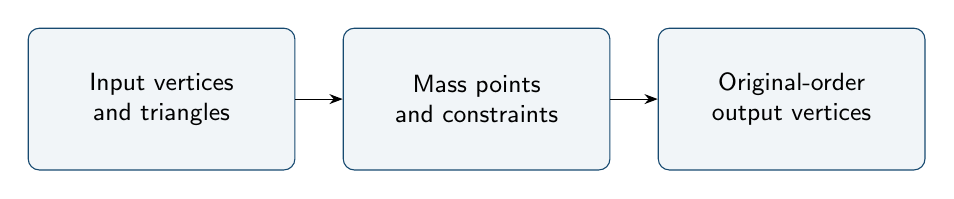
\begin{tikzpicture}[node distance=6mm,every node/.style={draw=vveblue,rounded corners,fill=vvelight,text width=0.26\linewidth,align=center,minimum height=18mm,font=\small\sffamily}]
\node (a) {Input vertices and triangles};\node (b) [right=of a] {Mass points and constraints};\node (c) [right=of b] {Original-order output vertices};
\draw[-{Stealth}] (a)--(b);\draw[-{Stealth}] (b)--(c);
\end{tikzpicture}\end{center}

The pinned positions decide which points stay fixed. The constructor also turns the cloth by a tiny angle, so a perfectly flat cloth can start to move in all directions. So the very first positions are slightly different from your input. In every physics step, each cloth does its own number of smaller steps (substeps). In each small step it slows the points a little (damping), adds gravity, guesses the new positions, corrects the constraints, and handles contacts with bodies and the floor. Cloth gets gravity automatically, unlike bodies. Compliance means softness. The engine divides it by the small step length squared, so it is not the same as a spring stiffness. More substeps make the cloth more exact, but cost more time.

\subsection*{Always use generateVertices}
Give your renderer the output of generateVertices(). It has one position per original corner, in your order. The inner list of mass points has fewer entries and a different order.
\source{modules/VPE.ixx; modules/VPE.cpp; examples/physicsexample/physicsexample.cpp}

\lesson{Cloth and bodies push each other}\label{vpe-core-18}
A body reacts to the cloth in the same step. Cloth looks at the bodies near it. Because it makes several small steps, it blends the body's old and new position for each small step, so it can follow a moving body. This is special for cloth: bodies among themselves do not get this treatment. When a cloth point touches a body, the overlap is shared by mass: a light point moves more, a heavy body moves less. The push and the friction change the point's speed and also the body's speed and spin.

\textbf{While the cloth moves}: After all cloth has moved (still in the same step)

\textbf{Collect the pushes for each body}: Move and turn the body by the collected amounts.

\textbf{Collect position corrections}: Apply the position corrections.

\textbf{Use the body's old and new position}: Update the body's matrices if it moved.

\textbf{Solve cloth constraints and contacts}: Clear the collected values for the next step.

So a cloth can push or pull a body right away, not one frame later. If you trace a body's final position in the debugger, look after the cloth part of the step. applyTransformation(matrix, simulate) moves a cloth. With simulate = false the whole cloth simply jumps. With true, pinned and free points move by different amounts (set by movementSimulation), so the cloth swings and bends as if it were carried.

\subsection*{Cleaning up cloth}
Cloth has its own list in the world. clear() does not remove cloth and does not call its erase callbacks: use clearCloths().
\source{modules/VPE.ixx; modules/VPE.cpp; examples/physicsexample/physicsexample.cpp}

\clearpage\part{Building a game with it}
\lesson{Get the code and build it}
\label{vpe-core-19}The earlier console-project section gives a small CMake integration. To run the repository's own checks, first clone the repository, then choose your platform's standalone build script. For example, on Linux:\begin{lstlisting}
git clone https://github.com/hlavacs/ViennaPhysicsEngine.git
cd ViennaPhysicsEngine
./build_linux.sh release --without-vve
\end{lstlisting}
On macOS use \api{./build_macos.sh release --without-vve}. On Windows use \api{.\build_windows.cmd release --without-vve} from a suitable PowerShell. The scripts print the configured standalone build directory and run its registered tests. Keep a separate build directory if you change compiler, platform, numeric configuration or rendering mode.

\api{VPE_BUILD_EXAMPLES} defaults to ON and adds the graphical example. Set it to OFF for a console-only integration. \api{VPE_BUILD_TESTS} defaults to OFF; the standalone script enables it. \api{VPE_VVE_IN_TREE} controls building VVE with VPE and defaults to ON on Windows. \api{VPE_DOUBLE_ACCURACY} and \api{VPE_FORCE_LEFT_HANDED} are OFF by default.

The graphical example needs additional prerequisites: the neighbouring VVE checkout, its dependencies and a compatible module toolchain. Building VVE in-tree needs CMake 3.31.8 or newer and Ninja. Follow the current VVE README for the Vulkan SDK and platform setup. On macOS use KosmicKrisp for the VVE path.

The default Windows workflow builds the libraries together. Linux and macOS can consume VVE's prebuilt module tree; the Linux script currently expects its Release build. Matching the compiler and standard-library/module options matters. If module compatibility errors appear, confirm those settings before trying to copy a compiled module manually.
\source{CMakeLists.txt; README.md; build_linux.sh; build_macos.sh; build_windows.cmd}
\lesson{A falling body}
\label{vpe-core-20}Save this complete program as \api{main.cpp} in the console project described earlier. It checks a physical result, rather than only whether construction succeeds.% doc-example: vpe_falling_cube_manual
\begin{lstlisting}
#include <cmath>
#include <iostream>
#include <memory>
import VEPhysicsEngine;

int main() {
    using W = vpe::VPEWorld;
    W world;
    int owner = 1; // A stable address used as an identity.
    auto body = std::make_shared<W::Body>(
        &world, "cube", &owner, &W::g_cube,
        glmvec3{1, 1, 1}, glmvec3{0, 3, 0},
        glmquat{1, 0, 0, 0}, glmvec3{0}, glmvec3{0},
        1.0_real, 0.0_real, 0.6_real);
    W::Force gravity;
    gravity.m_accelW = {0, world.c_gravity, 0};
    body->setForce(0, std::move(gravity));
    world.addBody(body);
    const auto start = body->m_positionW.y;
    for (int frame = 0; frame < 120; ++frame)
        world.tick(1.0 / 60.0);
    const auto y = body->m_positionW.y;
    const bool ok = std::isfinite(y) && y < start
                 && y > 0.4_real && y < 0.7_real;
    std::cout << "falling_cube ok=" << ok << " y=" << y << '\n';
    world.clear(); // Owner and world are still alive here.
    return ok ? 0 : 1;
}
\end{lstlisting}
A one-metre cube rests with its centre near y = 0.5. The slight offset comes from the collision margin. This test uses a broad tolerance and checks that the number is finite. Exact final digits are not a portability guarantee.
\lesson{Keeping objects alive}\label{vpe-core-21}
Plan who owns what before you add callbacks. The engine stores the address of your game object. If the object moves in memory, the address is wrong. This happens, for example, with a std::vector<GameObject> that grows. Use std::vector<std::unique\_ptr<GameObject>> instead: the pointers move, but the objects stay where they are.

\textbf{Object}: Must stay alive...

\textbf{VPEWorld}: as long as any body or cloth uses it.

\textbf{Polytope (shape)}: as long as any body uses it.

\textbf{Your game object (owner)}: until its body or cloth is removed and no callback uses it anymore.

Body shared\_ptr                              is shared by the world, your game object, contacts and joints.

\textbf{Visible object and mesh}: as long as move callbacks write into it.

\textbf{Everything a callback captures}: until the callback is removed or can no longer be called.

A shared\_ptr only keeps the body alive. It does not keep the owner, the shape or anything your callbacks use alive. A good design: each game object stores its body and its visible object together, and a scene class owns the world and the shapes. Shut down in this order: stop calling tick; call clearCloths() while the visible cloth still exists; call clear() while erase callbacks can still reach your game and renderer; then delete the scene, the shapes and finally the world.

\subsection*{clear() is not a full reset}
clear() removes bodies and joints, but not cloth, and it does not reset the clock or the floor. For a completely fresh start, delete the world and create a new one.
\source{modules/VPE.ixx; modules/VPE.cpp; examples/physicsexample/physicsexample.cpp}

\lesson{Connecting the renderer}\label{vpe-core-22}
Your code copies physics results to the visible objects. Load 3D models, materials and textures with the Vienna Vulkan Engine or your own loader. Create the collision shape separately. A box model can use g\_cube. A complex model usually needs a few convex shapes that you choose. Loading a model does not create a physics body.

\begin{center}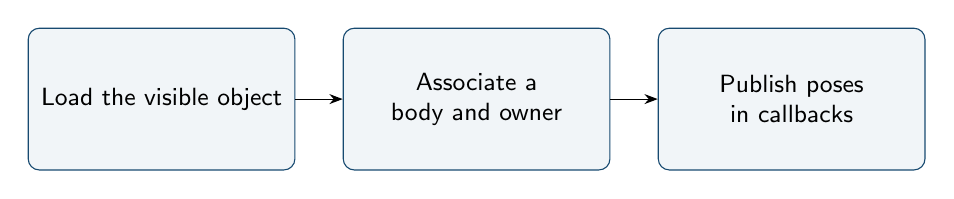
\begin{tikzpicture}[node distance=6mm,every node/.style={draw=vveblue,rounded corners,fill=vvelight,text width=0.26\linewidth,align=center,minimum height=18mm,font=\small\sffamily}]
\node (a) {Load the visible object};\node (b) [right=of a] {Associate a body and owner};\node (c) [right=of b] {Publish poses in callbacks};
\draw[-{Stealth}] (a)--(b);\draw[-{Stealth}] (b)--(c);
\end{tikzpicture}\end{center}

\begin{lstlisting}
// publishModel is YOUR function that moves the visible object.
body->m_on_move = [publishModel](double leftover,
                                  std::shared_ptr<W::Body> b) {
    auto p = b->m_positionW;
    auto q = b->m_orientationLW;
    publishModel(W::Body::computeModel(p, q, b->m_scale));
};
// Also set m_on_erase, to remove the visible object.
\end{lstlisting}

The simplest start is to copy the physics position as it is, like above. If you later use the leftover time to guess a smoother position, do not write that guess back into the body. For cloth, copy the output of generateVertices() into the mesh, and recalculate the normals if needed. Your renderer copies the data to the graphics card and draws it. VPE never touches the graphics card.

\subsection*{The floor you see and the floor that collides}
A textured plane in the Vulkan engine only shows a floor. The physics floor is always at y = 0. Put your visible floor there, or objects will seem to float or sink.
\source{modules/VPE.ixx; modules/VPE.cpp; examples/physicsexample/physicsexample.cpp}

\lesson{Physics in the game loop}\label{vpe-core-23}
When your game writes, when physics runs, when the screen reads.

\begin{lstlisting}
// One frame of your game. All of these are YOUR functions,
// except world.tick.
pollInput();
updateGameplay(elapsed);
applyQueuedPhysicsCommands();
if (!paused)
    world.tick(elapsed);
processQueuedCollisionEvents();
processQueuedObjectRemoval();
updateCameraAndUI(elapsed);
drawScene();
\end{lstlisting}

The order matters. Game rules set forces before the physics step. The callbacks publish new positions during tick. Adding and removing objects happens after tick. Then the scene is drawn.

If the Vulkan engine already runs the main loop, call tick from your update function there, with the elapsed time it gives you in seconds. Do not start a second loop.

\textbf{Situation}: What to do

\textbf{Pause and continue}: Do not call tick while paused. Do not pass the paused time afterwards.

\textbf{Stepping in the debugger}: Pass a small fixed time, or use debug mode (section~\ref{vpe-core-11}).

\textbf{A very slow frame}: Decide on a maximum elapsed value, for example 0.1 seconds.

\textbf{Changing the step rate}: Change m\_sim\_frequency and m\_sim\_delta\_time together.

\textbf{Several threads}: Only one thread may use the world at a time. The world is not thread-safe.

\subsection*{Measure before you change settings}
Watch the frame time, how many steps each tick does, the solver time and the number of bodies and cloths. A slow frame causes more catch-up steps, which can make the next frame slow too.
\source{modules/VPE.ixx; modules/VPE.cpp; examples/physicsexample/physicsexample.cpp}

\lesson{Forces, jumps and direct changes}\label{vpe-core-24}
Steady pushes, one-time pushes and editing values by hand. Steady pushes like gravity, an engine or wind are forces. Give each kind its own ID number, for example 0 for gravity, 1 for the player's engine and 2 for wind, so they do not overwrite each other.

\begin{lstlisting}
W::Force thrust;
thrust.m_accelW = glmvec3{3, 0, 0};
body->setForce(1ul, std::move(thrust));
// When the player lets go of the key:
body->removeForce(1ul);
\end{lstlisting}

A jump or a hit is a one-time push. Do not use a force for it, because a force stays. Instead, change the speed directly, for example body->m\_linear\_velocityW.y += 5;. Then check that the body really starts moving: there is no separate "wake up" function. If you change body values by hand, the engine's stored values may no longer fit:

\textbf{You changed...}: Then also...

\textbf{position or rotation}: call updateMatrices(), and move the body to its new grid cell if it moved far.

\textbf{size or inverse mass}: call inertiaTensorL() and updateMatrices().

\textbf{the position by a lot (teleport)}: remove and re-add the body, so the grid and contacts are correct.

\textbf{the shape}: keep the old and new shape alive, and recalculate inertia and matrices.

\subsection*{Easier: remove and create again}
For a reset or a respawn, it is often easier to remove the body and create a new one than to change many values. Do it outside tick, and add the forces, callbacks and joints again.
\source{modules/VPE.ixx; modules/VPE.cpp; examples/physicsexample/physicsexample.cpp}

\lesson{Collision events and deleting objects}\label{vpe-core-25}
Turn engine callbacks into safe game events. Register a collision callback for a body with addCollider(body, callback). When that body touches something, the callback gets two bodies: first your body, then the other one. Use their m\_owner to find your game objects. The other body may be the floor, whose owner is nullptr.

\begin{lstlisting}
// Only write the event down here; handle it after tick.
world.addCollider(body,
    [&events](std::shared_ptr<W::Body> mine,
              std::shared_ptr<W::Body> other) {
        events.push_back({mine, other});
    });
\end{lstlisting}

events is your own list, for example a std::vector of pairs. It keeps the bodies alive, but not their owners, so empty the list before you delete game objects. The callback can be called in many steps in a row for the same pair, and not in every step for objects that lie still. If you need "started touching" and "stopped touching", keep your own list of touching pairs and compare it from frame to frame.

\textbf{Step}: Why

\textbf{1. In the callback: only write down the event}: The engine is in the middle of its lists.

\textbf{2. Let tick finish}: Contacts and cloth must be completely done.

\textbf{3. Call eraseBody(body)}: This also removes the body's joints.

\textbf{4. Remove the visible object and the owner}: The erase callback must be able to finish its work first.

\textbf{5. Throw away old events}: So no later code uses a deleted owner.
\source{modules/VPE.ixx; modules/VPE.cpp; examples/physicsexample/physicsexample.cpp}

\lesson{Building a mechanism}\label{vpe-core-26}
Check the connection points and axes on screen. Start with two bodies and one joint: an unmovable support (inverse mass 0) and one moving part. Give the connection point in world coordinates at the place where the parts should meet. Hinges and sliders also need an axis that points the right way and is not zero.

\begin{lstlisting}
auto hinge = std::make_shared<W::HingeJoint>(
    support, door, hingePoint, glmvec3{0,1,0});
hinge->enableLimit(-1.0_real, 1.0_real);   // radians
hinge->enableMotor(0.5_real, 2.0_real);    // speed, maximum force
world.addConstraint(hinge);
// Stop the motor but keep the hinge:
hinge->disableMotor();
// The door breaks off:
world.removeConstraint(hinge);
\end{lstlisting}

For a hinge, the motor speed is a turning speed; for a slider it is a sliding speed. The maximum force is a limit for the solver, not an exact model of a real motor. Read the comments in the joint's code before you use real motor values. Draw small debug markers at both connection points and a line along the axis. Check that the movement looks right before you add more parts. Build chains and rag dolls one joint at a time. Very different masses, limits that fight each other, and shapes that block the movement all cause problems.

\subsection*{When it shakes}
Check the connection point, the axis direction, overlapping shapes at the start, the mass ratio, the time step and the number of solving rounds before you make the correction stronger. A stronger correction can hide the problem for a while but makes things more unstable.
\source{modules/VPE.ixx; modules/VPE.cpp; examples/physicsexample/physicsexample.cpp}

\lesson{Adding cloth}\label{vpe-core-27}
Keep the physics cloth and the visible mesh connected.

\begin{lstlisting}
// vertices, triangleIndices and pinnedPositions come from your mesh loader.
auto cloth = std::make_shared<W::Cloth>(
    &world, "banner", &bannerObject,
    onClothMove, onClothErase,
    vertices, triangleIndices, pinnedPositions,
    0.1_real, 8, 0.8_real);
world.addCloth(cloth);
// In onClothMove(leftover, clothPtr):
//     publishPositions(clothPtr->generateVertices());
// To remove it:
world.eraseCloth(&bannerObject);
\end{lstlisting}

Types: vertices and pinnedPositions are std::vector<glmvec3>, triangleIndices is std::vector<uint32\_t>. The move callback gets a double and a std::shared\_ptr<W::Cloth>; the erase callback gets only the shared\_ptr. publishPositions is your own function. Pinned positions must match corners of the mesh within the constructor's position tolerance. Corners within the position tolerance are joined, so check the seams of your model. The constructor throws an exception for bad input, so create cloth while loading, not in the middle of a frame.

\textbf{Setting}: What to test

\textbf{Substeps}: Better contacts against more CPU time.

\textbf{Bending compliance}: How much the cloth folds and bends.

\textbf{Damping}: How fast the cloth calms down.

\textbf{Friction and bounciness}: How cloth slides on and bounces off bodies.

\textbf{Movement simulation}: How free points follow when you move the cloth with applyTransformation.

Start with a small mesh with a pinned top edge. Check gravity, the corner order and cleaning up first. Add contacts with bodies and moving the cloth later. The cloth does not collide with itself.
\source{modules/VPE.ixx; modules/VPE.cpp; examples/physicsexample/physicsexample.cpp}

\lesson{Speed and stability}\label{vpe-core-28}
\textbf{Change one thing at a time, and measure. If you...}: you get...; but...

\textbf{raise the step rate}: smaller, more exact steps; more steps per second cost more CPU time.

\textbf{raise the solving rounds}: steadier contacts and joints; each step takes longer.

\textbf{have a heavy scene in real-time}: the time limit stops solving early; results get less exact. mode

\textbf{use bigger grid cells}: fewer missed pairs; more pairs to test.

\textbf{use more cloth substeps}: better cloth contacts; more CPU time.

\textbf{use a finer cloth mesh}: smoother cloth; more points, constraints and contacts.

\textbf{keep warm starting on}: stable stacks with less work; check that resting stacks really stay still.

Measure normal gameplay and the worst case. A test with only falling cubes does not tell you how a stack, a chain of joints or a cloth on a moving body behaves. Count pairs and contacts, not only bodies: a few bodies that overlap a lot can be slower than many bodies that are far apart. Many values belong together: step rate and step time, mass and inertia, position and matrices and grid cell, cloth softness and substeps. Do not change one of them without the others. Save the settings together with your test scenes, so you can repeat a test later.

\subsection*{A small set of test scenes}
Keep five scenes: a falling cube, a stack of boxes, a box on a slope, a hinge or slider, and a cloth touching a body. Write down positions, speeds and joint errors over time, not only whether the program still runs.
\source{modules/VPE.ixx; modules/VPE.cpp; examples/physicsexample/physicsexample.cpp}

\lesson{Troubleshooting}\label{vpe-core-29}
\textbf{Find the first place where the values go wrong. Problem}: Check first

\textbf{A body does not fall}: Inverse mass above 0? Gravity added? Does tick really do steps?

\textbf{The visible object does not move}: Is a move callback set? Does it move the right visible object?

\textbf{A body falls through another}: Did they become a pair (grid)? Too fast or too thin? Convex shape?

\textbf{Objects float or sink into the floor}: The physics floor is at y = 0. Move the visible floor there. Check units.

\textbf{Joints stretch or shake}: Connection point, axis, overlap, mass ratio, time step, correction, solving rounds.

\textbf{Cloth constructor throws}: Valid numbers? Triangle indices exist? Three per triangle? Substeps above 0?

\textbf{Cloth tears open at seams}: Use generateVertices() in the original order and check the mesh indices.

\textbf{Crash after deleting}: Owner, shape or callback data deleted too early? Removed with eraseBody(owner) while joints still exist?

\textbf{Long freeze after a pause}: A huge dt makes the engine catch up step by step.

\textbf{Picking selects strange bodies}: pickBody picks the body most in the look direction; it is not an exact ray test.

pickBody also crashes if there are no bodies at all, so check first. For exact picking, write your own ray test and then find the body by its owner. Print the values before and after the step where it goes wrong. If two bodies never become a pair, changing the friction cannot help. If the physics is right but the picture is not, more solving rounds cannot help: the problem is in the connection to the renderer.
\source{modules/VPE.ixx; modules/VPE.cpp; examples/physicsexample/physicsexample.cpp}

\lesson{Walking through the demo program}\label{vpe-core-30}
Follow one object from creation to the screen. Open examples/physicsexample/physicsexample.cpp. Start where the world and the Vulkan engine are created. Then find the function addCube (search for its definition), which creates a body. It makes a shared\_ptr with the world, a name, the game owner, the cube shape, size, position and material values. Then it sets the move and erase callbacks and adds gravity.

\begin{center}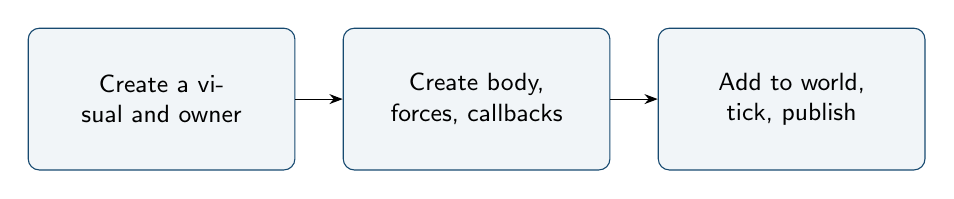
\begin{tikzpicture}[node distance=6mm,every node/.style={draw=vveblue,rounded corners,fill=vvelight,text width=0.26\linewidth,align=center,minimum height=18mm,font=\small\sffamily}]
\node (a) {Create a visual and owner};\node (b) [right=of a] {Create body, forces, callbacks};\node (c) [right=of b] {Add to world, tick, publish};
\draw[-{Stealth}] (a)--(b);\draw[-{Stealth}] (b)--(c);
\end{tikzpicture}\end{center}

Set a breakpoint in addBody and look at m\_bodies and the grid. In tick, notice the difference between one frame and one physics step. Step into broadPhase, narrowPhase and calculateImpulses only for the body you care about. Watch its speed change first, then its position. In the move callback, follow the owner back to the visible object. The callback calculates the matrix and hands it to the Vulkan engine, which draws it later. The physics engine stops at the callback. For cloth, find the make\_shared<VPEWorld::Cloth> call (search for its construction), then addCloth. Step into integrate and compare the generated positions with the order of the loaded mesh.

\subsection*{The demo works with old and new Vulkan engines}
The demo imports VVEngine (the current Vulkan engine) or VEEngine (older versions). CMake checks which one your Vulkan engine provides and sets VPE\_VVE\_USES\_VVENGINE. The physics module is always VEPhysicsEngine.
\source{modules/VPE.ixx; modules/VPE.cpp; examples/physicsexample/physicsexample.cpp}

\lesson{Quick reference}\label{vpe-core-31}
\textbf{The most important functions on one page. Task}: Use

\textbf{Create the world}: import VEPhysicsEngine; then vpe::VPEWorld world;

\textbf{Create a solid object}: std::make\_shared<VPEWorld::Body>(...) with a shape and an owner

\textbf{Add or remove it}: addBody(body), eraseBody(body)

\textbf{Push it}: setForce(id, force), removeForce(id)

\textbf{React to movement}: m\_on\_move, m\_on\_erase

\textbf{React to collisions}: addCollider(body, callback)

\textbf{Connect two bodies}: a joint in a shared\_ptr, then addConstraint / removeConstraint

\textbf{Create cloth}: std::make\_shared<VPEWorld::Cloth>(...), addCloth, generateVertices

\textbf{Move time forward}: tick(seconds)

\textbf{Clean up}: clearCloths() and clear(), in that order

Next steps: start with the falling cube from section~\ref{vpe-core-20}. Then add, one at a time: a renderer (section~\ref{vpe-core-22}), the game loop (section~\ref{vpe-core-23}), collision events (section~\ref{vpe-core-25}), joints (section~\ref{vpe-core-26}) and cloth (section~\ref{vpe-core-27}). The test file tests/vpe\_compile\_check.cpp contains more small examples of bodies, joints and cloth.

\subsection*{What a finished game integration has}
Owners and shapes that stay alive, only convex collision shapes, a clear game loop, callbacks that copy positions to the screen, changes made only after tick, a clean shutdown, and a few test scenes you can repeat.
\source{modules/VPE.ixx; modules/VPE.cpp; examples/physicsexample/physicsexample.cpp}

\clearpage\part{Detailed practice and current behaviour}\lesson{Work through force, acceleration and mass}
Suppose a body has mass two kilograms and you apply a world-space force of ten newtons to the right. Its acceleration from that force is five metres per second squared: force divided by mass. After a tenth of a second, its rightward speed has increased by about half a metre per second. The exact trajectory also depends on contacts and the integration steps.

Now give the same force to a one-kilogram body. Its acceleration is ten, so it gains speed twice as quickly. This is why a heavy crate feels harder to push. Gravity is usually entered as acceleration instead: every freely falling body receives approximately 9.81 metres per second squared downward, regardless of its mass.

\api{Force::m_accelW} adds acceleration directly in world space. \api{m_forceW} is a world-space force affected by inverse mass. \api{m_forceL} and \api{m_positionL} describe a local force and where it acts relative to the body. A force away from the centre can also make the body turn. Turning response depends on inertia, which describes how mass is distributed around the axes.

Use separate force IDs for separate causes. For example, reserve 0 for gravity, 1 for a player's thruster and 2 for wind. Replacing ID 1 changes the thruster without removing gravity. Remove only that ID when input ends. Do not add another ID every frame: that creates many simultaneous persistent forces.

A direct velocity change is convenient for an arcade jump. It is a change in metres per second, not a force in newtons. If you want a mass-dependent impulse response, your game must convert the impulse to a velocity change using inverse mass. Keep that decision explicit so game tuning has clear units.
\source{modules/VPE.ixx: Force; Body::setForce; Body::stepVelocity}
\lesson{Trace time across several frames}
By default the world uses a 60 Hz fixed interval: about 0.016667 seconds. Your application still passes actual elapsed seconds to \api{tick}. The world advances whole slots to catch up and keeps a remainder. The comparison is strictly greater than the next slot boundary. Do not expect a call at exactly one interval to advance exactly one slot on every floating-point boundary.

Imagine three frame durations: 0.008, 0.008 and 0.020 seconds. The first two together are still below one default interval. A movement callback may run, but no full slot has advanced. After the third, total time is 0.036 seconds; the engine can perform two full intervals, leaving a small remainder. Callback count therefore does not measure physics-step count.

The movement callback receives the remainder once the world finishes catching up. Start with the current solved pose. Later you may display a smoother estimated pose or interpolate stored poses. Keep that display state separate: writing it back into the body changes the next physical calculation and can make a resting object drift.

Pause by omitting physics ticks while continuing your user interface if needed. On resume, begin with fresh elapsed time. For a debugger pause or a very slow frame, choose a deliberate catch-up policy. Clamping to 0.1 seconds drops some real time; processing every elapsed second may freeze the application while it catches up. Neither policy should happen accidentally.

Changing \api{m_sim_frequency} alone does not recompute every dependent field. The default \api{m_sim_delta_time} was initialized from the original frequency. Configure the related values coherently before the first tick, and start with the default while learning. For repeatable exercises use fixed input sequences and numerical tolerances; the contact solver also has a wall-clock work limit.
\source{modules/VPE.ixx: VPEWorld clock fields; tick; calculateImpulses}
\lesson{A safe lifecycle from spawn to shutdown}
At spawn, first create a stable game owner and any custom shape. Then construct its body, assign callbacks and persistent forces, and add it to the world. Create joints only after their bodies are ready. Keep ownership in one scene or game layer so removal has a clear order.

During a tick, callbacks should record intent: copy a pose, append a small event, or request a later removal. They should not erase bodies, owners or constraints from a container the world may still be traversing. After the tick, process those requests. If several contacts request the same removal, combine them into one request before erasing.

On removal, keep the owner and renderer objects alive while \api{eraseBody(body)} calls its erase callback. Remove the visible object and game owner after that operation has finished. Clear queued events that still contain owner pointers. A shared body pointer in an event keeps the body alive, but cannot make a deleted owner address valid again.

For whole-scene shutdown: stop calling tick; call \api{clearCloths()}; call \api{clear()}; release visible objects and callback data; release custom shapes and remaining body pointers; finally destroy the world. Choose an order that lets every callback finish using its dependencies.

\api{clear()} is not a factory reset. It removes rigid bodies, contacts and constraints but leaves cloth and the clock state. For a genuinely new simulation session, destroy the old world after cleanup and create another world. This is simpler than manually guessing which clock fields need resetting.
\source{modules/VPE.ixx: addBody; eraseBody overloads; clear; clearCloths}
\lesson{A complete hinge exercise}
This program creates a small static support and a thin dynamic door. The hinge anchor is a point in world space; its axis points up. A zero axis cannot define a hinge. The example checks construction, stepping and cleanup with finite output. It does not claim to measure the accuracy of every hinge angle.% doc-example: vpe_hinge
\begin{lstlisting}
#include <cmath>
#include <iostream>
#include <memory>
import VEPhysicsEngine;

int main() {
    using W = vpe::VPEWorld;
    W world;
    int supportOwner = 1, doorOwner = 2;
    auto support = std::make_shared<W::Body>(
        &world, "support", &supportOwner, &W::g_cube,
        glmvec3{0.2_real}, glmvec3{0, 3, 0});
    auto door = std::make_shared<W::Body>(
        &world, "door", &doorOwner, &W::g_cube,
        glmvec3{1, 2, 0.1_real}, glmvec3{0.6_real, 3, 0},
        glmquat{1, 0, 0, 0}, glmvec3{0}, glmvec3{0},
        1.0_real);
    world.addBody(support);
    world.addBody(door);
    auto hinge = std::make_shared<W::HingeJoint>(
        support, door, glmvec3{0.1_real, 3, 0},
        glmvec3{0, 1, 0});
    hinge->enableLimit(-0.5_real, 0.5_real);
    world.addConstraint(hinge);
    for (int frame = 0; frame < 30; ++frame)
        world.tick(1.0 / 60.0);
    const bool ok = std::isfinite(door->m_positionW.x)
                 && std::isfinite(door->m_positionW.y);
    world.removeConstraint(hinge);
    world.clear();
    std::cout << "hinge ok=" << ok << '\n';
    return ok ? 0 : 1;
}
\end{lstlisting}
Next, give the door a small initial angular velocity or enable a motor. Record its pose over time and show the anchor and axis as debug lines in your renderer. If the parts begin overlapping, solve that placement before increasing the solver correction strength. Large mass ratios and constraints that fight one another are common sources of shaking.
\lesson{A complete cloth exercise}
This example creates four input vertices and two triangles. Indices start at zero: triangle \api{0,2,1} refers to three entries in the point vector. The top two positions become pins. Pins identify positions, not input index numbers.% doc-example: vpe_cloth_manual
\begin{lstlisting}
#include <cmath>
#include <cstdint>
#include <iostream>
#include <memory>
#include <vector>
import VEPhysicsEngine;

int main() {
    using W = vpe::VPEWorld;
    W world;
    int owner = 2;
    std::vector<glmvec3> points{
        {-1, 3, 0}, {1, 3, 0}, {-1, 2, 0}, {1, 2, 0}};
    std::vector<uint32_t> triangles{0, 2, 1, 1, 2, 3};
    std::vector<glmvec3> pins{points[0], points[1]};
    auto cloth = std::make_shared<W::Cloth>(
        &world, "small flag", &owner,
        W::callback_move_cloth{}, W::callback_erase_cloth{},
        points, triangles, pins, 0.1_real, 8, 0.8_real);
    cloth->m_stretch_compliance = 1.0e-3_real;
    world.addCloth(cloth);
    for (int frame = 0; frame < 60; ++frame)
        world.tick(1.0 / 60.0);
    auto output = cloth->generateVertices();
    bool ok = output.size() == points.size();
    for (const auto& p : output)
        ok = ok && std::isfinite(p.x) && std::isfinite(p.y)
                && std::isfinite(p.z);
    std::cout << "cloth ok=" << ok
              << " vertices=" << output.size() << '\n';
    world.clearCloths();
    world.clear();
    return ok ? 0 : 1;
}
\end{lstlisting}
The output restores the original input order. This matters for imported meshes with duplicated seam vertices. Physics may merge near-coincident corners into one mass point while the renderer still needs separate vertices for texture coordinates or normals. Keep the mesh's original index buffer and update its positions in that original order.
\lesson{Tune cloth without mixing up the controls}
The constructor's compliance argument controls bending. Its default is 1, while the example explicitly chooses 0.1. The number of substeps defaults to 4; the example chooses 8. A substep is a smaller interval within one fixed world slot. More substeps make contact and constraints cost more work, so measure them on your intended mesh.

The current public \api{m_stretch_compliance} defaults to \api{1.0e-3_real}. It controls how much edge lengths can change. Bending compliance controls folding. Both are compliance values: larger means softer. They are scaled with the squared substep duration inside the solver. A value is not a percentage and not a spring strength that should be increased to stiffen the cloth.

\api{m_air_damping} defaults to 0.8, \api{m_air_damping_quadratic} to 0.06, and \api{m_constraint_damping} to 0.3. Air damping reduces motion; constraint damping reduces relative movement along constrained directions. Change one setting at a time and compare recorded output. Confirm the exact field names in the current source before copying an older tuning preset.

Cloth restitution defaults to zero and friction to 0.6. These influence contact response. They cannot repair malformed triangles or a wrong mapping back to the visible mesh. The movement-simulation constructor argument controls the effect of transforming the cloth, rather than replacing the stretch or bending controls.

The constructor validates input and can throw. Check finite coordinates, triangle count divisible by three, in-range indices, nonzero triangle area, no unused disconnected point and positive substeps. Position merging and pin matching use a small tolerance around one millionth of a length unit. Test seams and very small models in your chosen world units.
\source{modules/VPE.ixx: Cloth constructor; ClothConstraint::solve; Cloth::integrate; tests/vpe_compile_check.cpp}
\lesson{Understand cloth and body contact}
A moving cloth corner can cross a body boundary during one substep. Looking only at its final position can miss the crossing. The current cloth contact path uses swept tests against rigid bodies and records where the movement meets a surface. This improves contact handling but is not a promise that arbitrarily fast or tiny features are always resolved.

When cloth presses on a dynamic body, contact response exchanges momentum. A static body has zero inverse mass and does not move. A dynamic body can receive a velocity change and a position or angular correction. The world applies accumulated corrections in the same fixed slot before publishing the final matrices and callbacks. This is why a cloth-body test should examine both participants.

Start with a cloth above a static box. Check that corners stay finite and that the visible cloth uses generated positions correctly. Then make the box dynamic and compare its response with the same scene without cloth. Finally add lateral velocity and friction. Keep those tests small so the first failing step can be inspected.

Cloth does not provide general cloth self-collision. A folded sheet may pass through another part of itself. Use this limitation when choosing the educational scene and mesh. Reducing the timestep cannot add an algorithm that the engine does not contain.
\source{modules/VPE.ixx: Cloth::integrate; swept contact helpers; tick; tests/vpe_compile_check.cpp}
\lesson{Connect to the current VVE facade}
VPE and VVE solve different problems. VPE stores physical bodies and calculates poses. VVE stores render objects and draws them. Your game holds the association between a body and a public VVE object handle. That association belongs to the game; the physics engine does not need a concrete renderer class.

Use the official VVE facade: import \api{VVEngine}, create an engine and obtain its world and \api{RenderSystem}. Create a visible cuboid or imported scene through that facade. Keep your physics owner in stable storage beside the visible handle. In the physics move callback, convert the current physical position and quaternion into the public transform representation accepted by your VVE version.

Preserve rotation as well as position. Keep visual scale consistent with collision dimensions, and account for the body's small collision margin when exact pixels appear slightly different. A visible floor belongs at y = 0 for the built-in physics ground. Updating an imported asset or creating a visible plane does not create a collider.

Call \api{tick} from your game's existing VVE update hook with elapsed seconds. Do not add a second nested \api{run} loop. Process queued physics events after that call. For cloth, the renderer needs the original-order positions from \api{generateVertices()}, updated normals when appropriate, and an upload path supported by the renderer.

The repository's physics example contains compatibility code for more than one VVE generation. Study how data crosses the boundary, then use the facade supported by your own VVE checkout. Avoid copying internal rendering descriptors or hard-coded compiled module paths into a new game API.
\source{examples/physicsexample/physicsexample.cpp; ../ViennaVulkanEngine/src/RenderSystem.ixx; ../ViennaVulkanEngine/src/World.ixx}
\lesson{Collect evidence that helps you debug}
A useful test says what was measured, which input produced it and whether the result is acceptable. The falling-cube check prints a name, a success flag and its final height. When a check fails, also record the first frame where the value leaves its allowed range, plus position, speed and elapsed time.

For collisions, separate three questions. Did the broad phase propose the pair? Did the narrow phase find contact points? Did the solver apply a reasonable response? If there is no candidate pair, friction and restitution cannot help. If the physical state is correct but the picture is wrong, examine your rendering bridge rather than solver iteration count.

For joints, measure the distance between the intended anchors and check that the allowed axis has the expected direction. For cloth, check finite positions, pin drift, vertex count, original vertex ordering and the movement of any contacted body. Include invalid-input tests: those catch asset problems before an interactive scene starts.

Use fixed input sequences for regression tests and tolerances for numerical comparisons. The rigid-body solver also stops according to a wall-clock work budget, so exact final digits can vary with machine load. Save the commit, compiler, configuration, timestep and tuning values with the result. A screenshot is useful evidence for appearance, while text output makes numerical failures easier to locate.

Run the standalone registered tests after changing the library. Run the small complete examples after changing guide code. A successful compile proves that names and signatures fit; a numerical run is needed to check the behaviour the lesson promises.
\source{tests/vpe_compile_check.cpp; modules/VPE.ixx: calculateImpulses; tests/CMakeLists.txt}
\lesson{Follow a contact from approach to rest}
Picture a cube falling toward a floor. Before contact, gravity changes its downward velocity and the integration step moves its centre. The cube's lower corners approach y = 0. Once a corner enters the contact region, the engine builds contact information: where the surfaces meet, a surface-normal direction and a penetration measure.

A normal is a direction perpendicular to a surface. For the horizontal floor, the outward direction points up. The contact solver compares the bodies' movement at the contact point. It then calculates an impulse that opposes closing movement. The static floor remains fixed; the dynamic cube changes velocity. A contact impulse can push surfaces apart but does not glue them together.

Bounce comes from restitution. With zero restitution, the response aims to remove closing normal speed rather than return it as a large rebound. A positive value allows a rebound. Friction affects the sideways part of the movement, so a sliding cube loses horizontal speed. The amount of friction is limited relative to the normal response; it is not an arbitrary command that sets horizontal velocity to zero.

Rotation matters even if you only watch the centre. A corner contact away from the centre can turn the cube. The solver uses velocity at that corner, including the effect of angular velocity. Inertia tells it how strongly the body resists rotation about each axis. This explains why moving all mass farther from an axis makes a body harder to spin, even when total mass is unchanged.

Small overlap can remain after a discrete step. Bias and slop describe how the solver corrects that error without applying an unlimited correction to every tiny numerical difference. Too strong a correction can create visible energy and shaking; too weak a correction can leave deep overlap. First confirm units, shape placement and timestep before tuning correction parameters.

When the cube is resting, contacts can persist between steps. Warm starting reuses previous impulse estimates to begin the next solve closer to a useful answer. It does not mean the old velocity is copied back. Resting and damping logic help the body settle. A test should look at drift and speed over many steps, rather than interpreting one contact frame as proof of a stable rest.
\source{modules/VPE.ixx: ground contact; positionBias; warmStart; calculateImpulses; Body::stepVelocity}
\lesson{Make a collision event useful to gameplay}
A physical contact is a numerical fact. Damage, sound and removal are game decisions built from that fact. A collision callback gives you two body references. It does not automatically tell you that this is the first frame of a new collision or that the contact is strong enough to damage something.

Use the callback to append a compact event to your own queue. The event can hold the two shared body pointers or stable game identifiers. Handle that queue after tick returns. If you use owner pointers, remember that a queued event does not extend the owner's lifetime. Resolve and process events before deleting those owners, or use your game's explicit identifier validation.

Suppose a projectile touches a crate and then the floor during a catch-up tick. You may receive more than one event before gameplay processes removal. Decide which event wins and combine duplicate deletion requests. Marking an object for deletion is a game-state change; actual removal can happen once, after all relevant iteration has finished.

Repeated contact is different from collision onset. For a repeated scrape sound, ongoing contact may be useful. For a one-time impact sound, track a pair of stable object identifiers and a recent-contact policy. Because callbacks for resting pairs are not guaranteed every step, absence of a callback alone is not a complete separation test. A reliable enter/stay/exit feature needs its own verified contact-state design.

Ignore or handle the floor explicitly: its owner is null. Do not cast and dereference that pointer as if every body had a game object. Use the shared-pointer erase overload for a removed rigid body so attached constraints are cleaned up. Afterwards remove its render object and owner while keeping callback dependencies valid.

Test the game policy with a projectile, one target and the floor. Print event count, chosen target, removal count and the final number of live game objects. A successful physical collision does not prove the damage policy was executed exactly once; the game test must check that count itself.
\source{modules/VPE.ixx: addCollider; narrowPhase; eraseBody overloads}
\lesson{Reset, teleport and change a body deliberately}
Directly assigning a public field is easy, but that field may have dependent state. A position change affects the model matrix, its inverse, broad-phase cell placement and contacts from the previous location. A mass or size change affects inertia. A shape change affects geometry and pointer lifetimes. Treat these as related operations.

For a respawn, a simple reliable approach is to queue removal after tick, erase the old body and create a new one with the intended pose and properties. Assign its callbacks and gravity again, add it to the world, then recreate any intended joints. This is more explicit than retaining stale contacts and guessing which cached values need resetting.

If you deliberately edit a pose, call the relevant matrix update and refresh grid membership and contact state according to the actual implementation. A large teleport should not leave the body in its old grid cell. Removing and re-adding is often the clearest educational route, but remember that removal can invoke callbacks and remove joints.

Changing inverse mass requires a coherent inertia update. Do not turn a static body dynamic merely by setting one number if its dependent rotational data still represent the old state. Do the configuration outside tick and verify both a straight push and a small off-centre push afterwards.

Keep old custom collision shapes alive until no bodies use them. Their internal pointers refer to their own vertices, edges and faces. Copying a shape as an ordinary value or letting its storage move can invalidate those relationships. Build custom shapes in stable ownership and use simple shared shapes wherever that fits the game.

After any reset operation, run the falling-body, contact and joint checks relevant to the change. Record the first pose after respawn and confirm the owner address and visible handle identify the new object. This catches integration errors that a normal uninterrupted simulation never exercises.
\source{modules/VPE.ixx: Body::inertiaTensorL; updateMatrices; addBody; eraseBody; Polytope}

\end{document}
